\chapter{整合项目资源}
\section{整合项目资源概述}
项目整体管理围绕项目计划进行,主要过程有计划制定、计划执行和计划变更控制。
\begin{figure}[!h]
	\centering
	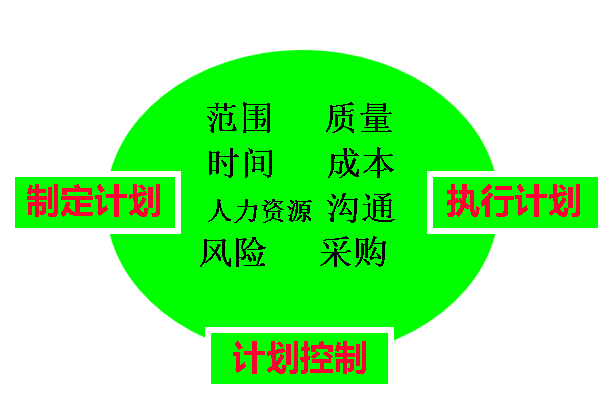
\includegraphics[width=0.6\textwidth]{image/3-1}
	\caption{项目整体管理主要过程}
\end{figure}
项目整体管理任务是在项目生命周期中协调所有其他项目管理知识领域所涉及的过程;它确保项目所有的组成要素在恰当的时间、正确的地方、合适的人物结合在一起,以成功地完成项目。
\subsection{整合项目资源的意义与作用}
项目整体管理将8大领域的相关要素结合在一起,随着项目沿着其生命周期演化,这些要素将变得更加集中。
\subsection{项目资源分析}
从静态的观点:人力资源、财务资源、项目实物资源。
\par 从动态的观点:非实物形式的生产资料、各种无形的管理约束、项目的运作过程。
\subsection{项目干系人分析}
项目干系人是指与项目相关的人,包括参与项目和受项目活动影响的人。
\subsection{IT项目项目经理}
项目经理是指承包方项目团队的项目经理,有时,采购方也会指派项目经理,或称为项目负责人,主要负责协调相关事务,采集需求,监控项目的进展等。
\subsubsection*{项目经理的职责}
确保项目目标实现;制定项目阶段性目标和项目总体控制计划;组织精干的项目管理班子;及时决策;履行合同义务,监督合同执行,处理合同变更。 
\subsubsection*{项目经理的主要权力}
指挥权;人事权;财权;技术决策权;设备、工具、材料的采购与控制权。
\subsubsection*{项目经理的素质要求}
良好的道德品质、健康的身体和心理素质、强烈的客户意识、专业的素质和素养、牢固的大局观、优秀的项目管理能力、强大的信心与坚强的意志、胆大、心细。
\subsection{高层管理人员的支持}
原因:
\begin{itemize}
	\item 获取足够的资源
	\item 项目经理需要一些特殊的审批
	\item 跨部门、跨组织的协调
	\item 项目经理需要得到高层管理人员的指导和帮助
\end{itemize}
\section{项目管理计划}
\subsection{项目管理计划的内容}
项目管理计划要记录计划的假设以及方案选择,要便于各干系人间的沟通,同时还要确定关键的管理审查的内容、范围和时间,并为进度评测和项目控制提供一个基准。
\par 项目计划包括:整体介绍、组织描述、管理程序、技术程序、任务范围、时间进度、经费预算等。
\par 项目的管理和方法主要包括:管理目标、项目控制、风险管理、项目人员、技术过程。
\par 项目任务主要包括:
\begin{itemize}
	\item 主要工作内容
	\item 主要可交付成果
	\item 工作有关的其他信息
\end{itemize}
\par 项目进度主要包括:进度概要、进度细要、与进度有关的其他信息。
\par 项目预算主要包括:预算概要、预算细要、其他信息。
\par 综上,项目管理计划的内容:介绍、项目组织、管理过程、技术过程、(工作包、进度和预算)。
\subsection{项目计划的制定方法}
制定原则:层次性、详略得当、符合现实、重视沟通。
\subsection{项目计划的管理过程}
\begin{figure}[!h]
	\centering
	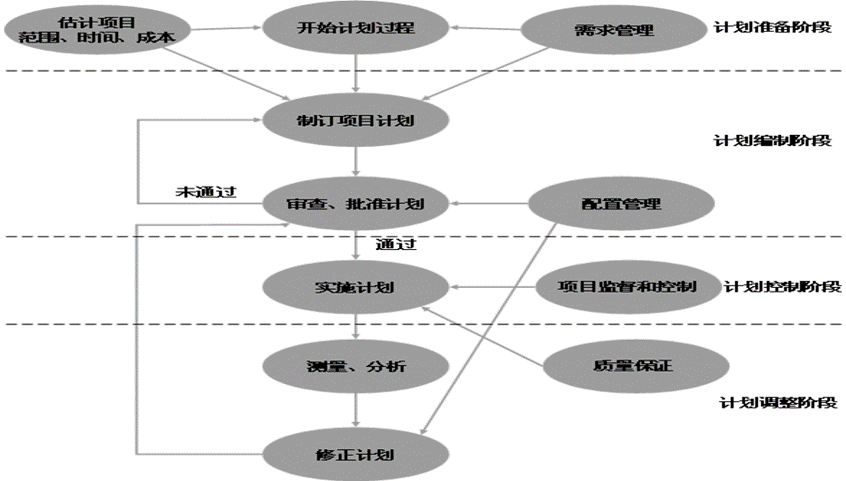
\includegraphics[width=0.8\textwidth]{image/3-2}
	\caption{项目计划的管理过程}
\end{figure}
\subsection{项目干系人的进一步分析}
项目管理的首要任务:全面识别出项目干系人及其在项目中的影响,从项目干系人的识别开始来分析和管理项目。
对干系人的分析步骤:
\begin{enumerate}
	\item 识别项目干系人 ;
	\item 分析项目干系人对项目的重要程度和影响程度;
	\item 分析项目干系人对项目的的支持程度。
\end{enumerate}
\subsection{实施项目管理计划}
项目整体管理将项目计划和项目执行视为互相渗透,不可分割的活动。
\par 适当改进项目计划。
\section{整体变更控制}
软件特殊性:动态性、灵活性、不确定性、易变性、隐蔽性、不可重复性、预计性和度量性差。
\par 整体变更控制:指在项目生命周期的整个过程中对变更进行识别、评价和管理,其主要目标是:
\begin{itemize}
	\item 对影响变更的因素进行分析、引导和控制,使其朝着有利于项目的方向发展;
	\item 确定变更是否真的已经发生或不久就会发生;
	\item 当变更发生时,变更进行有效的控制和管理。
\end{itemize}
\subsection{整体变更控制的输入和输出}
\begin{figure}[!h]
	\centering
	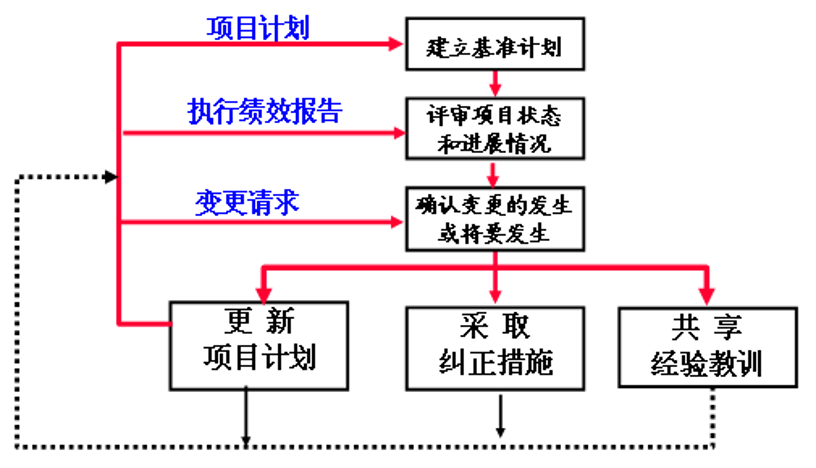
\includegraphics[width=0.6\textwidth]{image/3-3}
	\caption{项目整体变更控制}
\end{figure}
\subsection{整体变更控制的工具与技术}
\subsubsection*{变更控制系统}
变更控制系统指规定项目绩效如何监测与评估的一组正式的、有文件记载的程序。
\subsubsection*{配置管理}
配置管理用于确保项目产品描述的正确性和完整性。
\par 配置管理的主要工作:
\begin{itemize}
	\item 识别并记载对象或系统的功能和物理特性
	\item 控制特性的变更
	\item 记录并报告变更及实施状况
	\item 审核对象与系统,核实是否符合要求
\end{itemize}
\subsubsection*{管理整体变更控制的方法}
\begin{enumerate}
	\item 把项目管理视为一个不断地沟通和协商谈判的过程  
	\item 为变更制定计划    
	\item 建立正式的变更控制系统,包括变更控制委员会(CCB)    
	\item 运用配置管理    
	\item 制定一定的管理程序以实现较小变更的快速决策    
	\item 通过书面和口头的执行绩效报告确认和管理变更    
	\item 运用项目管理软件和其他软件协助进行变更管理和沟通
\end{enumerate}